\section{Isotropic\_Sqw: A general $S(q,\omega)$ coherent and incoherent scatterer}
\label{s:isotropic-sqw}
\index{Samples!Coherent and incoherent isotropic scatterer}
\index{Coherent and incoherent isotropic scatterer}
\index{Inelastic scattering}

\component{Isotropic\_Sqw}{V. Hugouvieux, E. Farhi}{Sqw$\_{coh}$, $\sigma_{coh}$, Sqw$\_{inc}$, $\sigma_{inc}, V_\rho, \sigma_{abs}, T$}{$q_{min}, q_{max}, \omega_{min}, \omega_{max}, d\phi$, order}{not fully validated}

\begin{figure}
  \begin{center}
    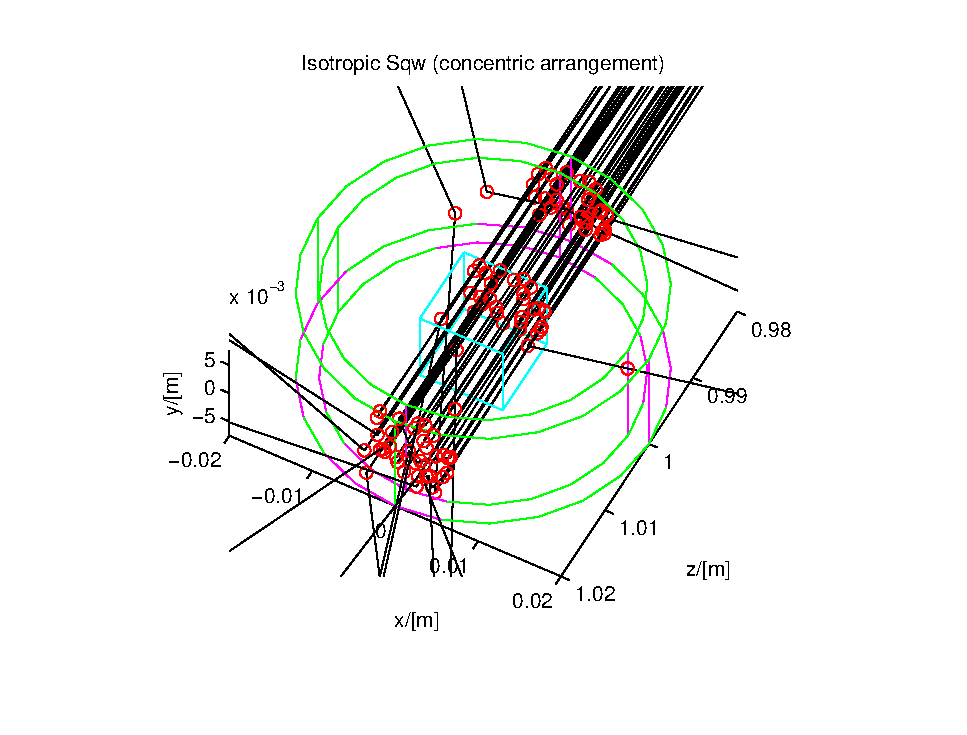
\includegraphics[width=0.9\textwidth]{figures/sqw.eps}
  \end{center}
\caption{An $l-^4$He sample in a cryostat, simulated with the Isotropic\_Sqw component in concentric geometry.}
\label{f:isotropic-sqw}
\end{figure}

The component assumes that the sample has the structure of an isotropic material. This stands for liquids, glasses (amorphous systems), polymers, gaz, and may be extended to powders.

\subsection{Neutron interaction with matter}

When a neutron enters a material, according to usual models and letting the absorption aside to begin with, it 'sees' atoms as disks with a surface equal to the total scattering cross section of material $\sigma$. Each coherent and incoherent process is associated with a given probability to hit these cross-sections, according to $\sigma_{coh}$ or $\sigma_{inc}$. We may choose randomly a scattering position along the path, using e.g. an expeonential decay probability. If the scattering condition is not satisfied, the neutron is transmitted, and leaves the sample. In any case, the absorption lowers the intensity according to an $e^{-\rho \sigma_abs} d$ absorption law along the propagation path. In this process, the neutron is considered to be a particule.

Once the neutron 'knows' that something (terrible) is going to occur, it looks for a possible excitation to interact with. Then we turn to the wave description of the neutron, which interacts with the whole volume. The distribution of excitations, from which derives their relative intensity in the scattered beam, is simply the dynamic structre factor - or scattering law - $S(q,\omega)$. According to the definition of the density of states, we may use $g(\omega)$ as the probability law to scatter at a given energy transfert.

The neutron leaves the scattering point when a suitable $(q, \omega)$ choice has been found to satisfy the conservation laws. The process is iterated until the neutron leaves the volume of the material, eventually producing multiple scattering contributions.

\subsection{Theoretical side}

Following Squires (\cite{squires}, p63), the neutron differential scattering cross section for both coherent and incoherent processes is
\begin{equation}
\frac{d^2\sigma}{d\Omega dE_f} = \frac{\sigma}{4\pi}\frac{k_f}{k_i} N S(q, \omega)
\end{equation}
with usual notations: $N=\rho V$ is the number of atoms in the scattering volume $V$ with density $\rho$, $E_f, E_i, k_f, k_i$ are the energy and wavevectors of final and initial states respectively, and $\sigma$ is the total scattering cross-section. The unit of the dynamical structure factor $S(q,\omega)$ is an inverse energy.

Some easely measureable quantities in a liquid are the \emph{static pair correlation function} $g(r)$ and the \emph{structure factor} $S(q)$, defined as:
\begin{eqnarray}
\rho g(\vec{r}) &=& \frac{1}{N} \sum_{i=1}^N \sum_{j \neq i} \langle \delta(\vec{r}+\vec{r}_i-\vec{r}_j) \rangle \\
S(\vec{q}) &=&\int S(\vec q,\omega) d\omega \\
           &=&1 + \rho \int_V [g(\vec{r})-1] e^{i\vec{q}.\vec{r}} d\vec{r} \\
           &=&1 + \rho \int_{0}^{\infty} [g(r)-1] \frac{\sin(qr)}{qr} 4 \pi r^2 dr {\rm\ in\ isotropic\ materials.}
\end{eqnarray}
Both $g(r)$ and $S(q)$ converge to unity for large $r$ and $q$ values respectively, and they are representative of the atoms spatial distribution. Moreover in a liquid $\lim_{q \rightarrow 0} S(q) = \rho k_B T \chi_T$ where $\chi_T=\frac{\partial \rho}{\partial P}_{V,T}$ is the compressibility \cite{Egelstaff67}. These quantities are obtained experimentaly from diffractometers.

On the other hand, we may measure, usually with time-of-flight instruments, the \emph{density of states} $g(\omega)$  which is the fraction of modes whose energy lie between $\omega$ and $\omega+d\omega$ \cite{lovesey84}
\begin{equation}
g(\omega) = \frac{\int S(q,\omega) dq}{\iint S(q,w) dq, d\omega} .
\end{equation}
This function is normalized to unity, $\int (gh(\omega) d\omega = 1$ and is a probability distribution of mode energies in the material.

The main idea to implement the scattering from $S(q, \omega)$ is to basically make two consecutive Monte Carlo choices, applying the well known \emph{joint probability} theorem:
\begin{equation}
P(q \cap \omega) = P(\omega).P(q \mid \omega) .
\end{equation}

Thus we define $P(\omega)$ as the cumulated distribution of the density of states $g(\omega)$.  $P(\omega)$ is the probability for an excitation to have an energy lower than $\omega$.

Similarly, we define the conditional probability $P((q \mid \omega)$ to be, for each energy lying between $\omega$ and $\omega+d\omega$, the cumulated distribution of the probability
\begin{equation}
\hat g(q,\omega) = \frac{S(q, \omega)}{\int S(q,\omega) dq} .
\end{equation}
$P(q \mid \omega)$ is the probability for an excitation to have a wavevector lower than $q$, for a given energy transfert $\omega$.

\begin{figure}
  \begin{center}
    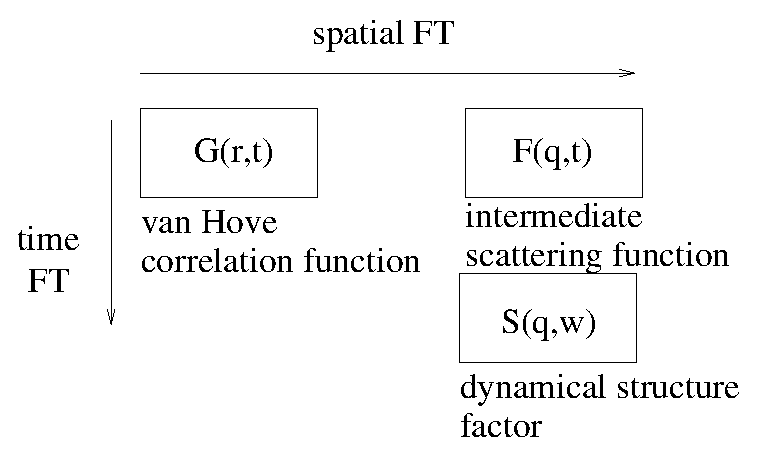
\includegraphics[width=0.9\textwidth]{figures/GFS.eps}
  \end{center}
\caption{The probability functions extracted from $S(q,\omega)$. The energy transfert is first selected from the density of states, then the wavevector is obtained from $\hat g$.}
\label{f:isotropic-sqw}
\end{figure}


\subsection{The implementation}
\subsubsection{Choosing the interaction position}

The probability that the neutron scatters between two positions $x$ and $x+dx$ is given by $\mu e^{-\mu x}dx$, where $\mu = \rho\sigma$ is the linear attenuation. If the straight path to the sample volume exit is $d_{out}$, the probability that the neutron scatters before exiting the sample at a distance $d_{scatt}$ is:
\begin{equation}
P(d_{scatt} < d_{out}) = \int_0^{d_{out}} \mu e^{-\mu x}dx = 1 - e^{-\mu d_{out}}. \\
\end{equation}
Form that law, we may compute the cumulated distribution, which gives the probability for scattering to occur at a distance lower than $d_{scatt}$. This law may be analytically inverted so that the path length $d_{scatt}$ may be obtained directly from a uniform distribution random number $\xi$
\begin{equation}
d_{scatt} = -\frac{1}{\mu} \ln(1 - \xi[1 -e^{-\mu d_{out}}]).
\end{equation}
Then we scale the neutron weight by $1 - e^{-\mu d_{out}}$, in order to account for the fraction of neutrons scattering before exiting the sample.

A similar method is used in the \verb+Single_crystal+ component (section \ref{s:Single_crystal}).


\subsubsection{Choosing the type of interaction}
\subsubsection{Choosing the $q$ and $\omega$ transfert}